%!TEX root = CS818_assessment.tex
\section{Overview of dataset}
The analysis in this study is based on a dataset from the UC Irvine Machine Learning Repository \cite{Obesity}, comprising 2111 observations across 17 variables collected from participants in Mexico, Peru and Colombia. Approximately 77\% of the data is synthetic, which was used to address an unbalanced distribution in obesity levels \cite{Palechor2019a}. The target variable is obesity level, labelled 'NObeyesdad' in the dataset. This categorises individuals based on their BMI into the groups Insufficient Weight, Normal Weight, Overweight Level I, Overweight Level II, Obesity Type I, Obesity Type II and Obesity Type III. The calculation for BMI is
\[
\text{BMI} = \frac{\text{Weight (kg)}}{(\text{Height (m)})^2}
\]
and obesity is defined as a BMI equal or greater to 30.00 in line with the World Health Organisation's definition \cite{Palechor2019a}. The coded variables that appear in the dataset are detailed in table \ref{tab:variables}.

\begin{table}[!h]
\centering
\begin{tabular}{|l|l|}
\hline
\textbf{Variable Name} & \textbf{Description} \\
\hline
family\_history\_with\_overweight & Family history of overweight \\
FAVC & Frequent consumption of high-caloric food \\
FCVC & Frequency of vegetable consumption in meals \\
NCP & Number of main meals per day \\
CAEC & Frequency of food consumption between meals \\
SMOKE & Smoking status \\
CH2O & Daily water consumption \\
SCC & Monitoring of daily calorie intake \\
FAF & Frequency of physical activity \\
TUE & Daily usage time of technological devices \\
CALC & Frequency of alcohol consumption \\
MTRANS & Usual mode of transportation \\
NObeyesdad & Obesity level \\
\hline
\end{tabular}
\caption{Variables and Descriptions}
\label{tab:variables}
\end{table}

\section{Exploratory analysis: results}

Figure \ref{fig:distributions} captures the distribution of the demographic variables, which shows a right-skew for age with a mean of 24.3 years and few entries from participants aged 40 and above. This could limit how well any findings generalise to older populations. Weight's distribution is unimodal and slightly right-skewed, with a mean of 86kg, whilst height's distribution is more symmetrical, with a mean of 1.7m.

\begin{figure}
  \centering
  \begin{subfigure}[b]{0.7\textwidth}
    \centering
    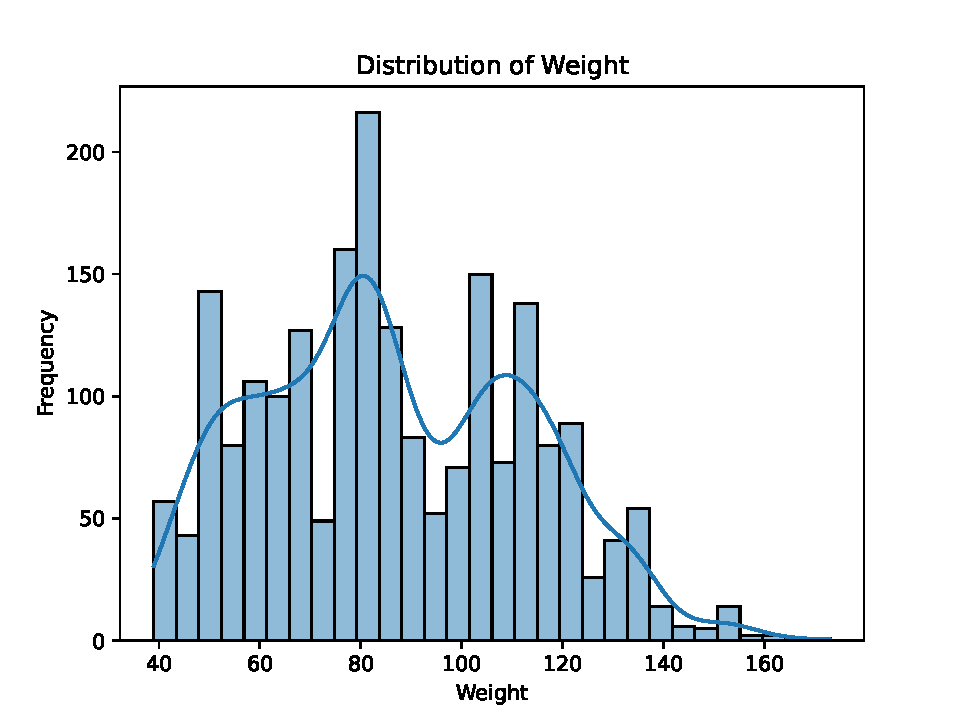
\includegraphics[width=\textwidth]{weight_dist.pdf}
    \label{fig:weight}
  \end{subfigure}
  \hfill
  \begin{subfigure}[b]{0.7\textwidth}
    \centering
    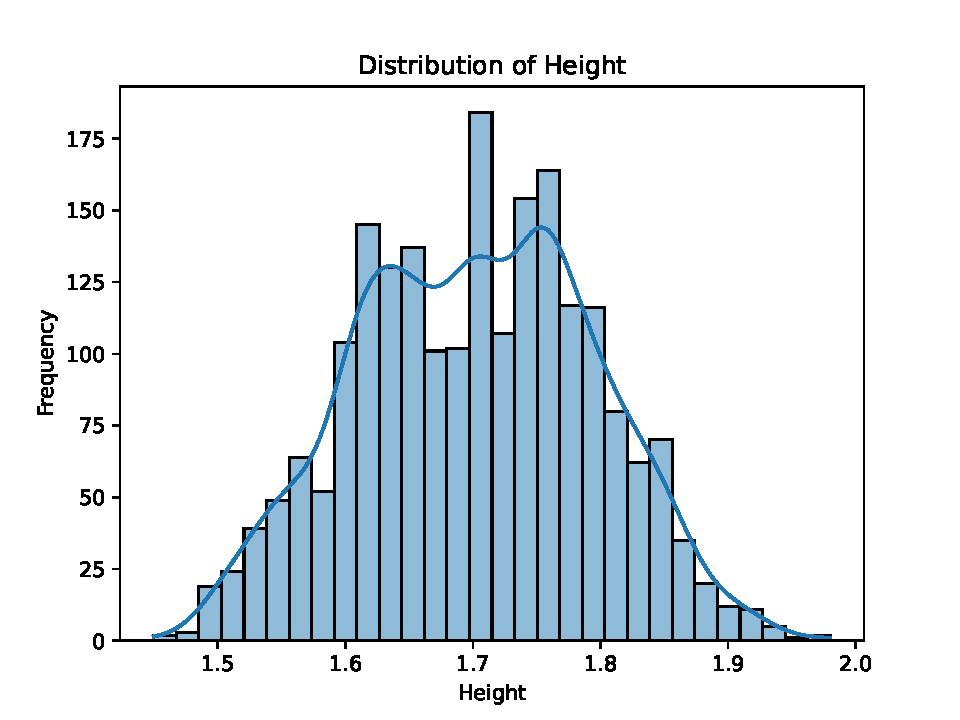
\includegraphics[width=\textwidth]{height_dist.pdf}
    \label{fig:height}
  \end{subfigure}
  \hfill
  \begin{subfigure}[b]{0.7\textwidth}
    \centering
    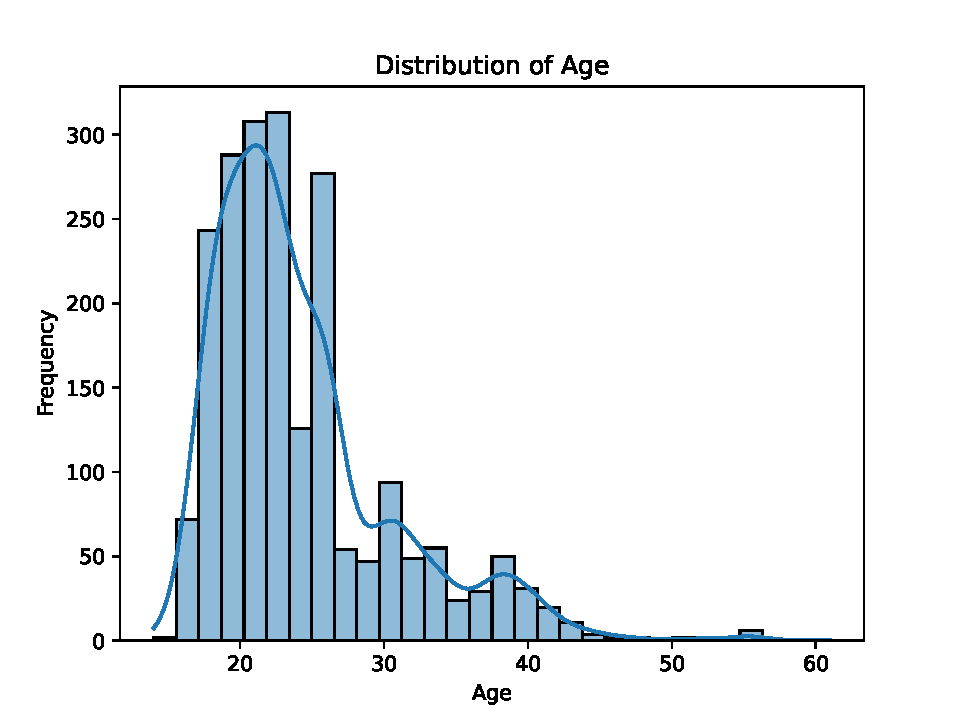
\includegraphics[width=\textwidth]{age_dist.pdf}
    \label{fig:age}
  \end{subfigure}
  \caption{Distributions of weight, height, and age.}
  \label{fig:distributions}
\end{figure}

Expanding out the exploratory analysis, we can consider the correlation between numeric variables. To ensure obesity rate is captured, the category 'BMI' will be added using the formula already given. And since BMI is calculated from height and weight, those categories will be removed to avoid duplication and to focus in on variables beyond body-measurements.

\begin{figure}
  \centering
  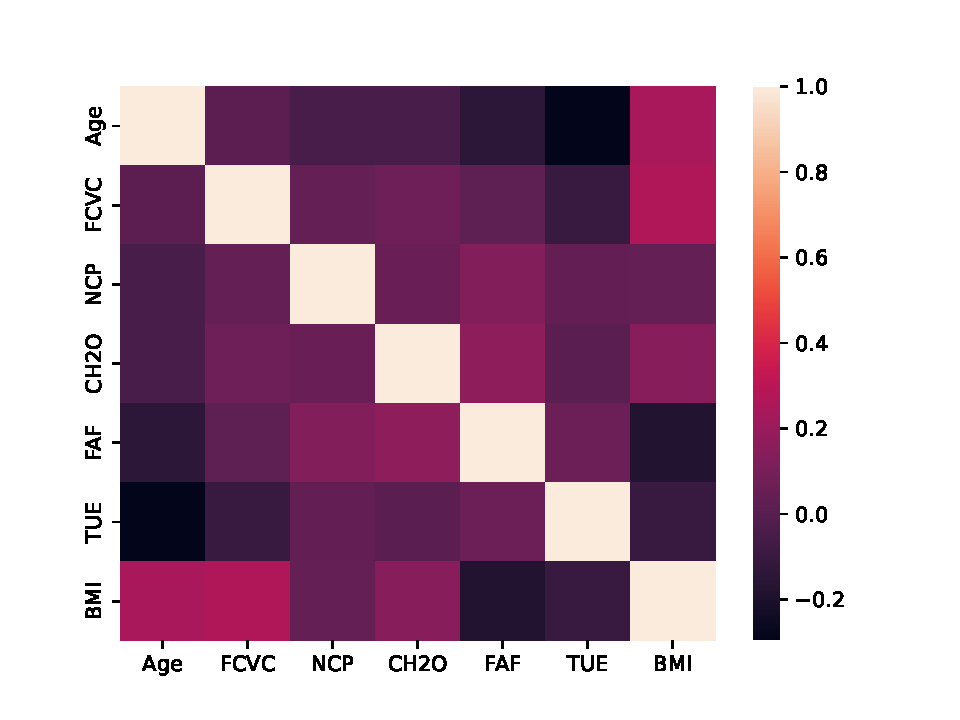
\includegraphics[width=0.8\textwidth]{numeric_correlations.pdf}
  \caption{Correlation Heatmap}
  \label{fig:heatmap}
\end{figure}

\begin{table}
\centering
\caption{Strongest Correlation Pairs}
\label{tab:top_correlations}
\begin{tabular}{llr}
\toprule
Variable 1 & Variable 2 &  Correlation \\
\midrule
Age        & TUE        &    -0.297 \\
BMI        & FCVC       &     0.264 \\
Age        & BMI        &     0.244 \\
BMI        & FAF        &    -0.178 \\
CH2O       & FAF        &     0.167 \\
Age        & FAF        &    -0.145 \\
BMI        & CH2O       &     0.144 \\
FAF        & NCP        &     0.130 \\
FCVC       & TUE        &    -0.101 \\
BMI        & TUE        &    -0.100 \\
\bottomrule
\end{tabular}
\end{table}

As per figure \ref{fig:heatmap} and table \ref{tab:top_correlations}, the strongest correlation is the negative relationship between age and time on electronic devices, though this relationship is not directly applicable to obesity. Of greater relevance are positive relationships between BMI and both vegetable consumption (FCVC) and age. There is also a negative relationship between BMI and physical activity (FAF), though in all cases the strength of the relationship is fairly weak. 

\FloatBarrier

The dataset also contains the categorical variables CALC (how often a respondent drinks alcohol) and CAEC (how frequently a respondent eats between meals). In both cases, the data is heavily concentrated in the 'Sometimes' category, though there were a reasonable number of respondents who noted they never drink alcohol, as per \ref{fig:calc_caec}. Similarly, the MTRANS (mode of transport) variable in figure \ref{fig:MTRANS_heatmap} shows the vast majority of respondents travelling by public transport, with a smaller minority travelling by automobile, and very few travelling by either bike, motorbike, or walking. In their current skewed form, these variables could disproportionately influence model estimates or clustering outcomes.

\begin{figure}
  \centering
  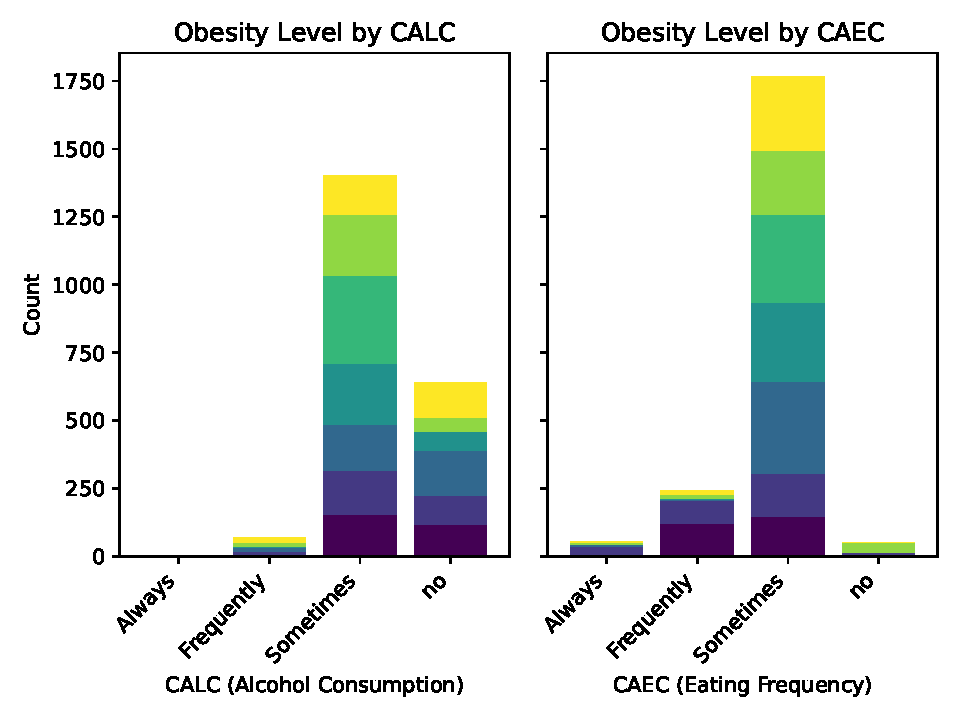
\includegraphics[width=0.8\textwidth]{CALC_and_CAEC.pdf}
  \caption{Distribution of Obesity Level by CALC and CAEC}
  \label{fig:calc_caec}
\end{figure}


For the final section of this exploratory analysis, we can consider how the binary variables relate to obesity levels. Here, 'Obese' follows the WHO definition as falling in category Obesity Type I, II and III, whilst 'Not obese' is all remaining categories, representing a BMI of below 30. As shown in figure \ref{fig:binary_obesity}, whilst an individual's gender or smoking status has little relation to obesity levels, individuals reporting a family history of obesity are significantly more likely to be obese than those with no such family history. Similarly, high consumption of calorific foods (FAVC) is perhaps unsurprisingly associated with higher obesity, and monitoring calories with lower obesity.   

\begin{figure}
  \centering
  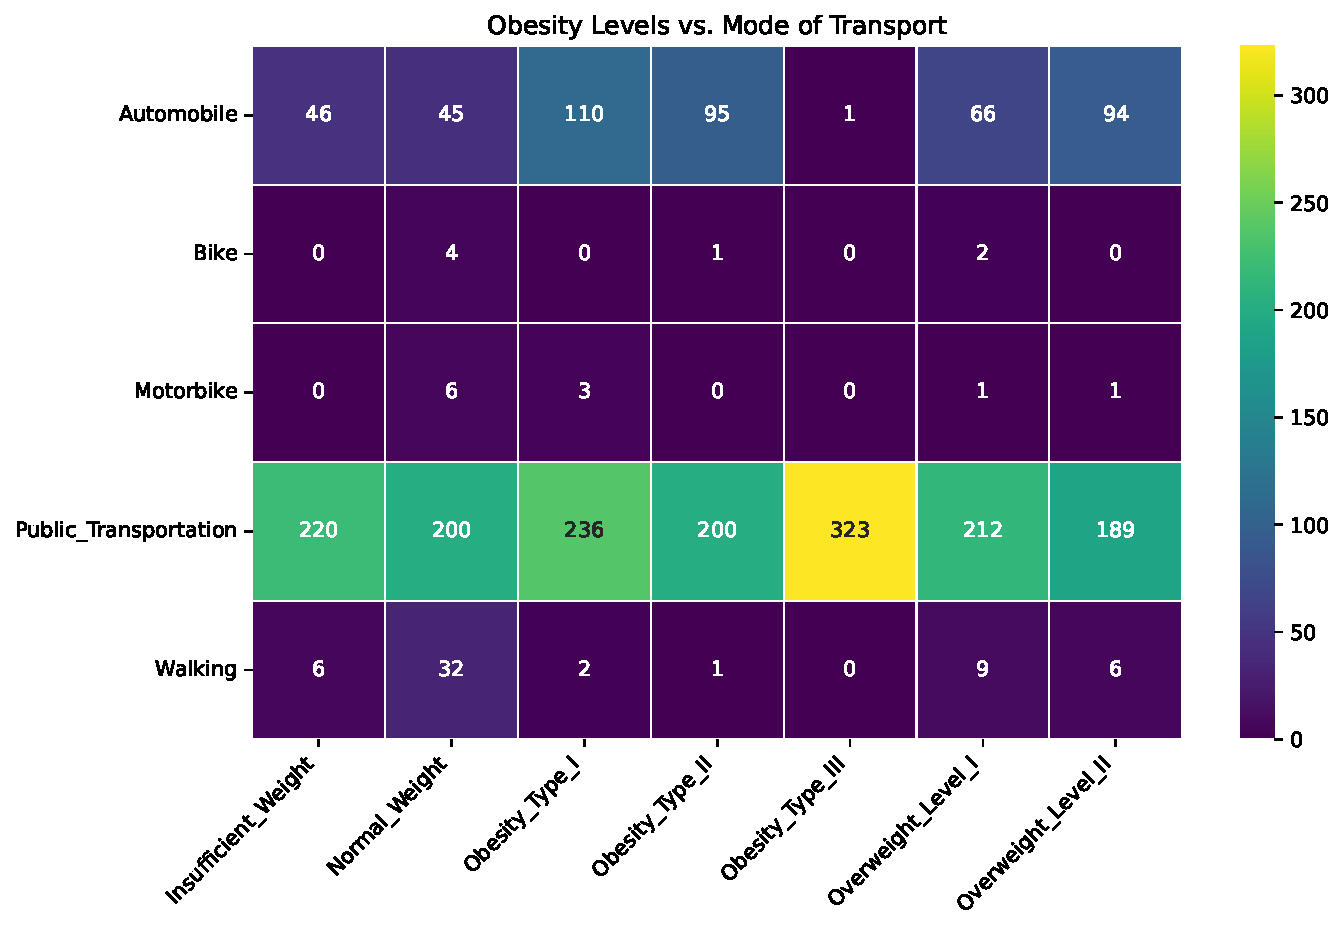
\includegraphics[width=1\textwidth]{MTRANS_heatmap.pdf}
  \caption{Obesity Levels vs. Mode of Transport}
  \label{fig:MTRANS_heatmap}
\end{figure}

\begin{figure}
  \centering
  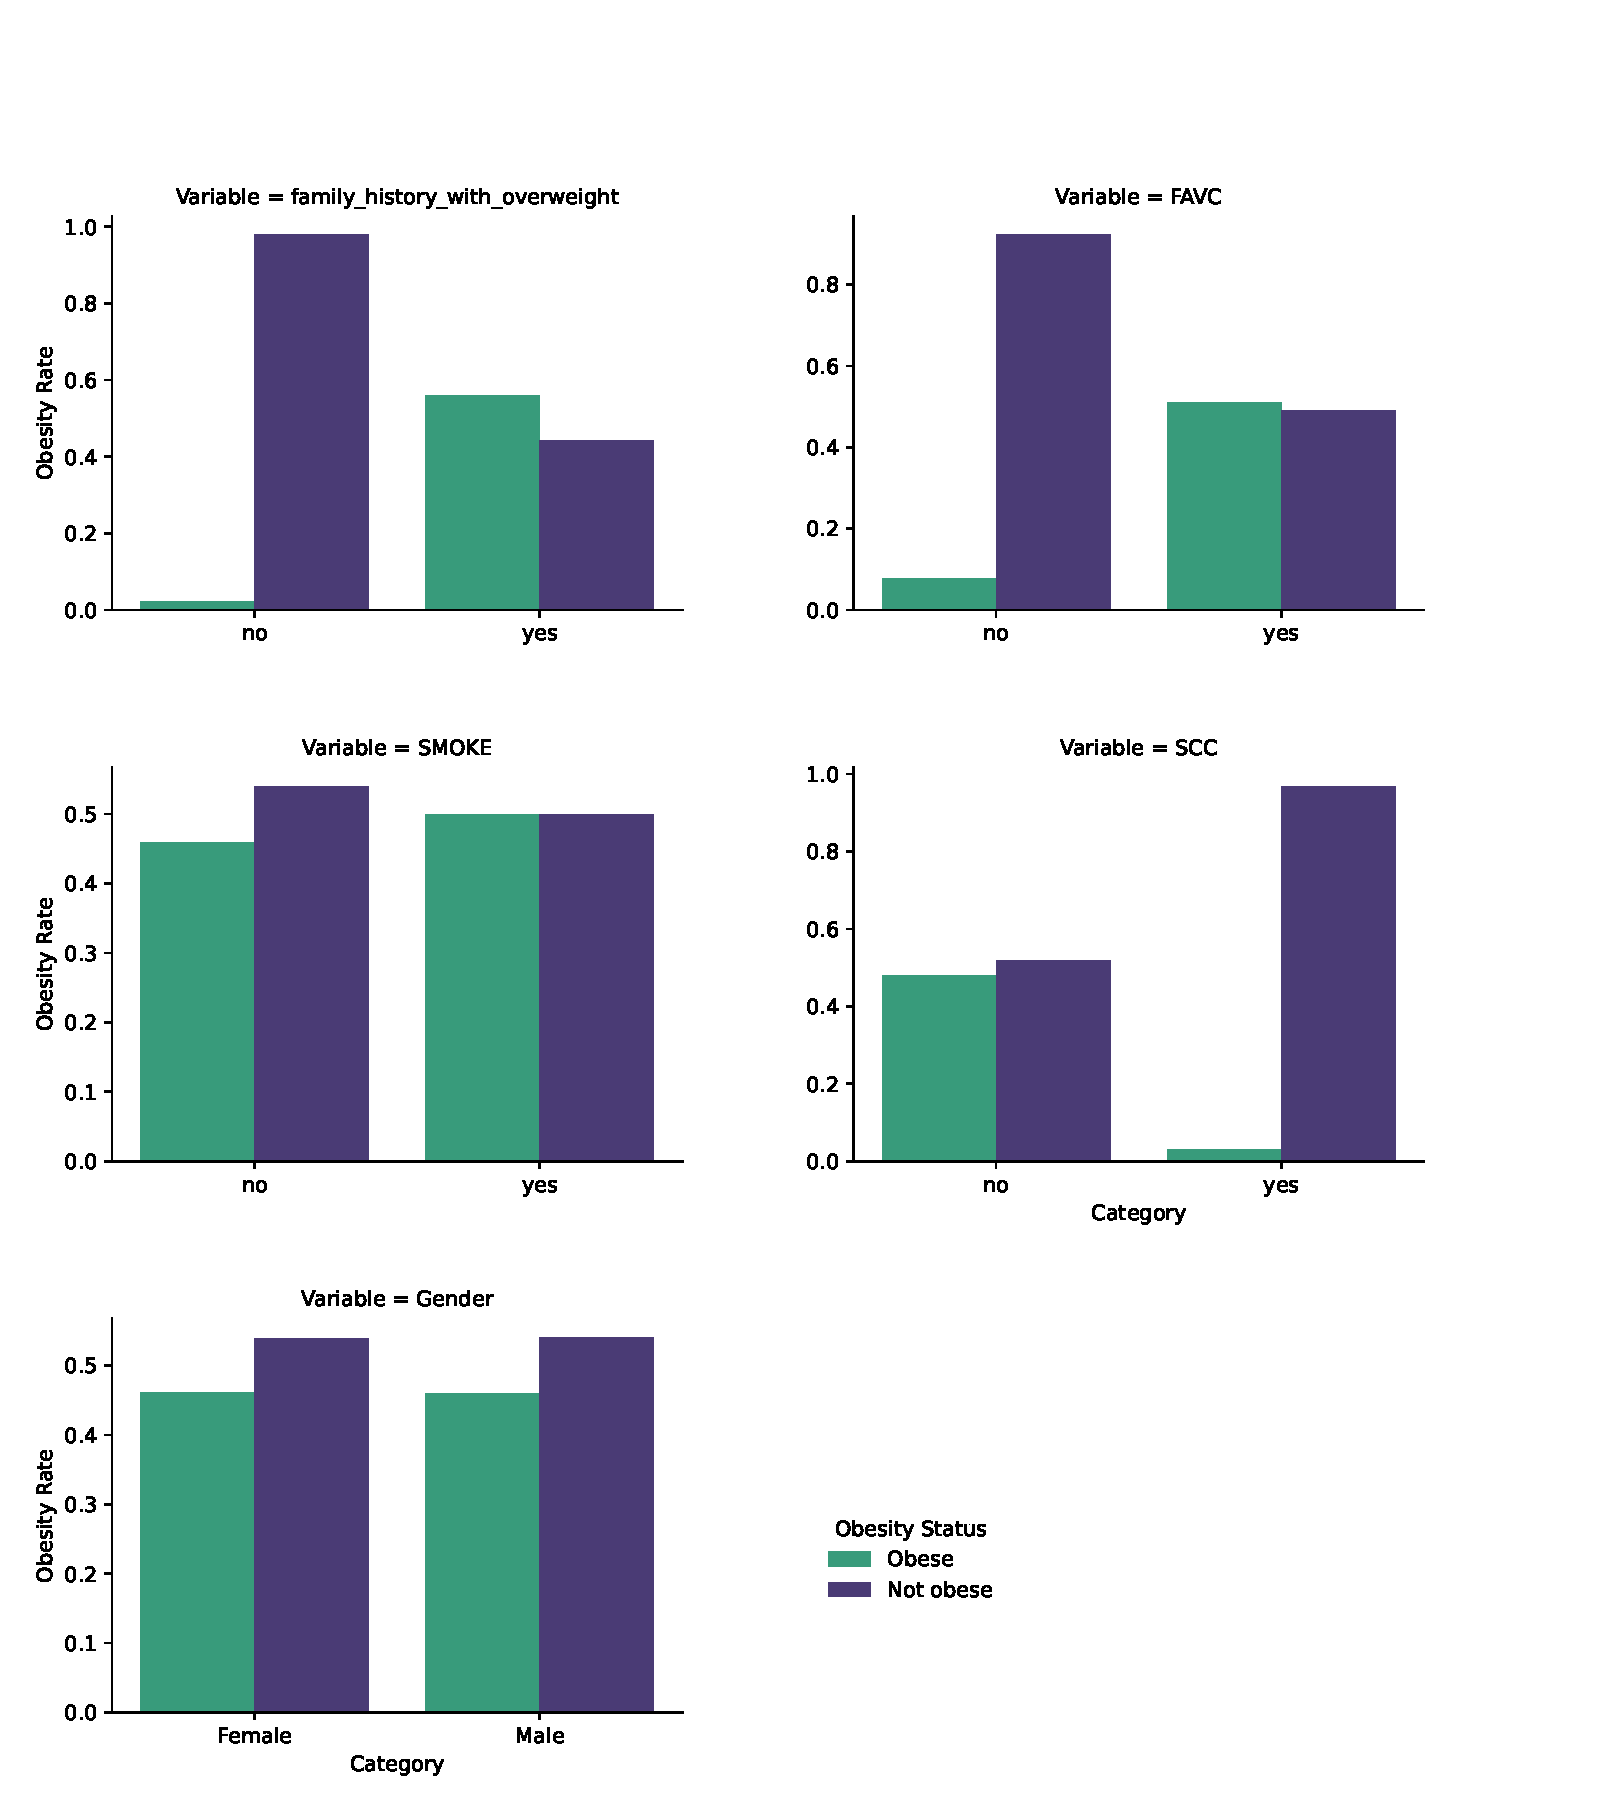
\includegraphics[width=1\textwidth]{binary_obesity.pdf}
  \caption{Obese vs. Not Obese for Binary Variables}
  \label{fig:binary_obesity}
\end{figure}

\FloatBarrier
\section{Discussion}

This initial exploratory analysis has provided a clear understanding of the dataset. Bivariate analysis was used to identify correlations. The link between low physical activity and higher BMI is consistent with research showing the positive impact exercise has on obesity risk \cite{Bergens2020}. Similarly, individuals may become more sedentary as they grow older, which could contribute to the link between age and BMI. However, the fact that higher vegetable consumption is correlated to higher BMI directly contradicts findings and public health advice which encourages greater vegetable consumption as a means of reducing obesity risk \cite{Nour2018}. This will be considered when conducting further analysis in the report's remaining sections. Similarly, analysis highlighted the concentration of responses to certain categorical variables such as alcohol consumption, which could indicate a predisposition amongst respondents towards particular behavioural patterns which will be borne in mind. Finally, the dataset is primarily made up of synthetic data. Whilst the SMOTE technique used by the creators is methodologically robust, there is always a risk with synthetic data that it fails to capture real-world variability \cite{Giuffre2023}. These potential limitations will be considered when evaluating the generalisability of any findings.

Whilst this approach has allowed us to uncover trends, univariate and bivariate analysis does not adequately capture the interactions between variables. For example, the correlation matrix shows a strong correlation between age and time on electronic devices, and separately between age and BMI, suggesting but leaving unexplored an interplay between these factors. To better understand potential interrelationships, more advanced multivariate techniques must be employed, which is the subject of the following section. 

